
\documentclass[paper=a4, fontsize=11pt]{scrartcl} % A4 paper and 11pt font size

\usepackage[T1]{fontenc} % Use 8-bit encoding that has 256 glyphs
\usepackage{fourier} % Use the Adobe Utopia font for the document - comment this line to return to the LaTeX default
\usepackage[german]{babel} % English language/hyphenation
\usepackage{amsmath,amsfonts,amsthm} % Math packages

\usepackage{lipsum} % Used for inserting dummy 'Lorem ipsum' text into the template
\usepackage[htt]{hyphenat}
\usepackage{sectsty} % Allows customizing section commands
\allsectionsfont{\centering \normalfont\scshape} % Make all sections centered, the default font and small caps
\usepackage{minted}
\usepackage{caption}
\usepackage{graphicx}
\usepackage[
  backend=biber,
  style=ieee
]{biblatex}
\usepackage{fancyhdr} % Custom headers and footers
\pagestyle{fancyplain} % Makes all pages in the document conform to the custom headers and footers
\fancyhead{} % No page header - if you want one, create it in the same way as the footers below
\fancyfoot[L]{} % Empty left footer
\fancyfoot[C]{} % Empty center footer
\fancyfoot[R]{\thepage} % Page numbering for right footer
\renewcommand{\headrulewidth}{0pt} % Remove header underlines
\renewcommand{\footrulewidth}{0pt} % Remove footer underlines
\setlength{\headheight}{13.6pt} % Customize the height of the header

\numberwithin{equation}{section} % Number equations within sections (i.e. 1.1, 1.2, 2.1, 2.2 instead of 1, 2, 3, 4)
\numberwithin{figure}{section} % Number figures within sections (i.e. 1.1, 1.2, 2.1, 2.2 instead of 1, 2, 3, 4)
\numberwithin{table}{section} % Number tables within sections (i.e. 1.1, 1.2, 2.1, 2.2 instead of 1, 2, 3, 4)

%\setlength\parindent{0pt} % Removes all indentation from paragraphs - comment this line for an assignment with lots of text

%----------------------------------------------------------------------------------------
%	TITLE SECTION
%----------------------------------------------------------------------------------------

\newcommand{\horrule}[1]{\rule{\linewidth}{#1}} % Create horizontal rule command with 1 argument of height

\title{	

\includegraphics[width=0.6\linewidth]{img/Mathnatlogo.png}\\[1cm]
\normalfont \normalsize 
\textsc{Master Praktikumsarbeit} \\ 
\textsc{Lehrstuhl für Betriebssystem und Rechnernetze} \\ [25pt]
\horrule{0.5pt} \\[0.4cm] 
\huge Grenzen der Leistungsfähigkeit und architektonische Beschränkungen der BlueField-3 \\ % The assignment title
\horrule{0.5pt} \\[1cm]
\author{Sten Heimbrodt} % Your name

\date{\normalsize\today} % Today's date or a custom date
}

\addbibresource{refs.bib}

\newpage
\begin{document}

\maketitle % Print the title

\tableofcontents
\newpage
\section{Einleitung}
% Allgemeiner und den Leser besser abholen. Was haben wir vor und was sind die Randbedingungen
% Alle Quellen des Projektes findet man...
Das Problem der Lastverteilung stellt eines der fundamentalsten in der Informatik dar. Viele Strategien und Ansätze prägen dabei die Landschaft der Implementierungen und variieren teils stark im jeweiligen Energieverbrauch. Seit geraumer Zeit begegnen Hersteller solchen Problemen mit technischen und architektonischen Lösungen. So entwickelt sich der Trend hin zu einer heterogenen Compute Landschaft. Die hier vorliegende Arbeit beschäftigt sich mit der Klasse der SmartNICs, im speziellen der BlueField-3 von Nvidia \cite{nvidia_bluefield_dpu}. 

Es werden technische Limitierungen anhand von Experimenten untersucht sowie ein gewisser Anteil an reverse Engineering betrieben, um Licht auf die Architektur zu werfen. Diese wird leider seitens Nvidia als proprietär betrachtet und dementsprechend nicht veröffentlicht. Außerdem wird die Flow API aus dem DOCA Framework verwendet, um die speziellen Hardwarebeschleuniger zu programmieren, die den eigentlichen energetisch Effizienten Vorteil bringen. Diese Arbeit versucht also ebenfalls, ein Verständnis für die API zu schaffen, um auch andere Probleme mittels DOCA Flow implementieren zu können. 

Ziel ist es, die technischen Limitationen, die so nicht im Material seitens des Herstellers genannt werden, zu ermitteln. Zentral wird im Rahmen dieser Projektarbeit der XenoFlow Loadbalancer vom ursprünglichen Zustand (Version 0.1), der in der Bachelorarbeit \cite{heimbrodt2025bluefield} entstanden ist, auf eine vollständige Major-Release Version 1.0 angehoben. Die ursprüngliche Version von XenoFlows wurde mittels DOCA Flow auf der Bluefield-3 implementiert, weshalb auch in dieser Arbeit auf derselben Plattform gearbeitet wurde. Alle Quellen des Projekts sind auf Github unter \url{https://github.com/gespel/XenoFlow} abgelegt.
\section{BlueField Architektur}
Bei der Bluefield-3 handelt es sich um eine Netzwerkkarte der Klasse der SmartNICs. Diese zeichnen sich dadurch aus, dass neben den Komponenten einer konventionellen Netzwerkkarte zusätzliche, herstellerseitig integrierte Hardwarebeschleuniger bereitgestellt werden. Außerdem wird im Falle der BlueField noch ein komplett eigener ARM-Host verbaut, der es ermöglicht, Anwendungen vollständig vom eigentlichen Host, in dem die BlueField verbaut ist, gekapselt auszuführen. 

Diese Beschleuniger decken unterschiedliche Funktionen ab und sind selbst keine klassischen Prozessoren, sondern entweder Application-Specific Circuits (ASICs) oder Field-Pro-gram-mable-Gate-Arrays (FPGAs). Der Vorteil solcher spezialisierter Hardware ist einerseits die enorm bessere Energieeffizienz und andererseits die daraus resultierenden Geschwindigkeitsgewinne. Das wird bei SmartNICs besonders offensichtlich, da es sich um eine sehr hochfrequente Verarbeitungspipeline handelt. Daher ist jegliche Verarbeitung von Daten auf Seiten der Netzwerkkarte verpflichtet, sämtliche Operationen derart zu modellieren, dass die Latenz in einem möglichst kleinen Umfang bleibt. Entscheidend ist es bei solchen Operationen, die absolute Anzahl an Taktzyklen möglichst gering zu halten oder sogar im optimalen Fall vollständig zu umgehen. Dabei setzen ASICs und FPGAs vor allem auf ihre großen Datenbusse, die dazu genutzt werden können, das Paket vollständig auf einen Datenpfad zu legen und entsprechend zu verarbeiten. Es wird dazu die Eigenschaft von klassischen Netzwerkpaketen ausgenutzt, dass Pakete meist an erwartbaren Bitpositionen die jeweiligen Informationen codieren. Eine weitere wichtige Unterscheidung, die für die späteren Experimente relevant ist, sind die beiden Datenpfadklassen \textbf{On-Path} und \textbf{Off-Path}. On-Path bedeutet im wesentlichen, dass alle zugehörigen Beschleuniger und Komponenten gezwungenermaßen immer an der Verarbeitung beteiligt sind. Im Umkehrschluss bedeutet dies allerdings auch, dass die Performance der On-Path-Komponenten direkten Einfluss auf die Datenrate hat. Off-Path-Komponenten hingegen können bei Bedarf in den kritischen Datenpfad integriert werden, um beispielsweise zusätzliche Funktionalität zu gewährleisten, wie das Parsen von bestimmten anderen Bitpositionen innerhalb des Pakets. Der besagte On-Path, also der kritische Datenpfad, ist in Abbildung 2.1 auf der rechten Seite über den Netzwerk Ein- und -Ausgang zu erkennen. Die entsprechenden Off-Path-Komponenten sind auf der linken Seite zu sehen und sind mittels PCIe Switch mit dem entsprechenden ARM-Host verbunden.
% neuere Version der Grafik
\begin{figure}
    \centering
    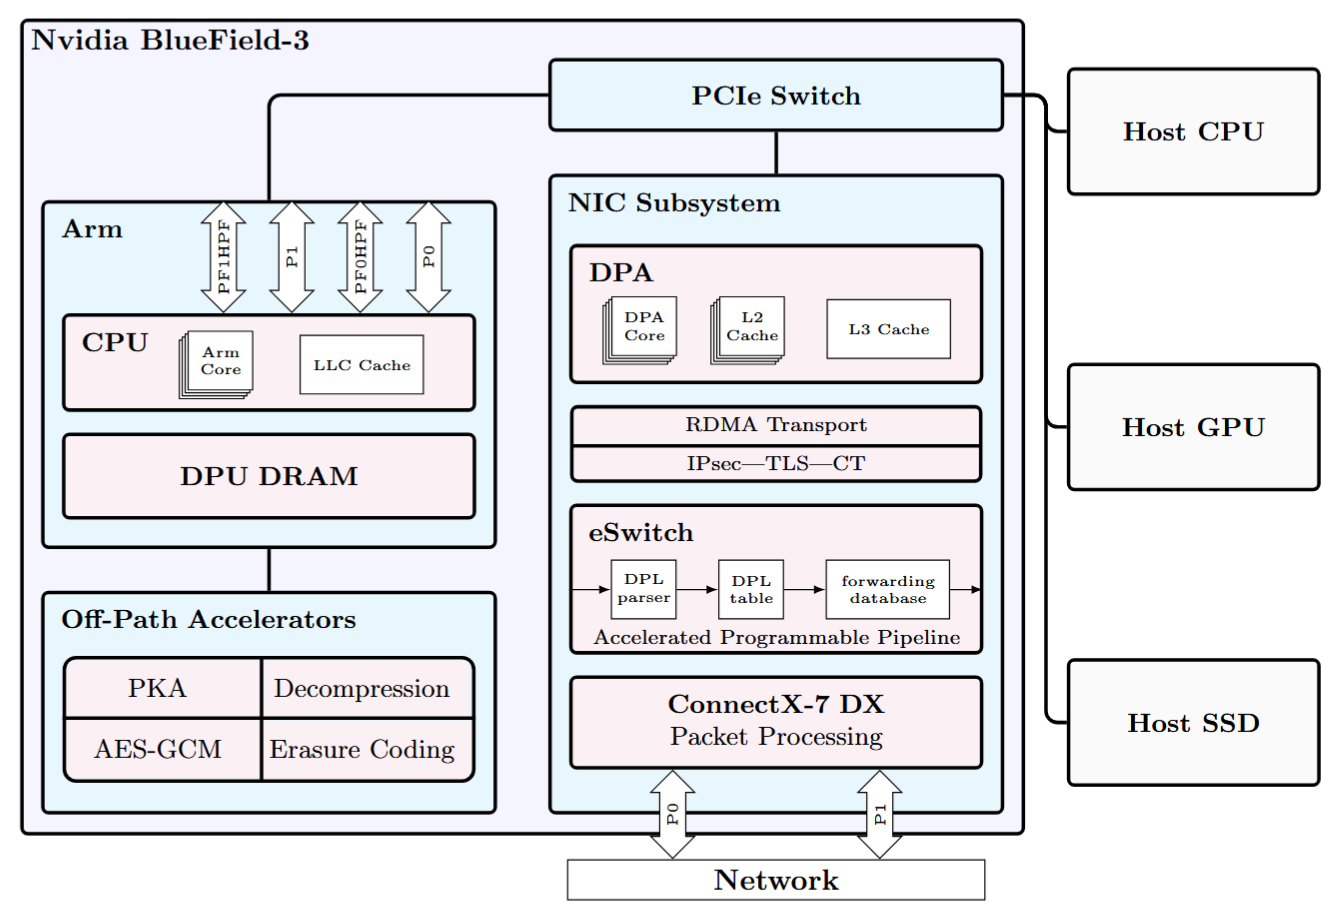
\includegraphics[width=1\linewidth]{img/bluefield.png}
    \caption{BlueField-3 Architektur \cite{schroetter2026xenoflow}}
    \label{fig:placeholder}
\end{figure}
\subsection{DOCA Flow}
Nvidia gibt der Kundschaft mit DOCA ein sehr mächtiges Werkzeug an die Hand, um selbst Anwendungen für die BlueField- sowie die ConnectX-Plattform zu entwickeln. Dabei bildet DOCA selbst einen Überbegriff für eine Menge von speziellen Bibliotheken, welche alle meist ein oder mehrere Funktionen eines Hardwarebeschleunigers abdecken. Für diese Projektarbeit ist das sogenannte \textbf{DOCA Flow} Framework verwendet worden. Es erlaubt die direkte Programmierung des \textbf{eSwitch} , welcher, wie in Abbildung 2.1 zu sehen, die erste und in speziellen Fällen auch die einzige ausgeführte Hardwareeinheit ist. DOCA Flow kann aus den üblichen Paketquellen des jeweiligen Linux Betriebssystems installiert werden und besteht aus offenen sowie teils kommentierten C-Header-Files mit vorkompilierten Shared-Object-Bibliotheken. Nvidia bietet außerdem eine Dokumentation sowie eine Reihe von Beispielen an, die entsprechend der Problemstellung als Implementierung vorliegen. Diese \textbf{Samples} werden ebenfalls mit DOCA Flow mitinstalliert.
\subsubsection{Pipes und Entries}
\begin{figure}
    \centering
    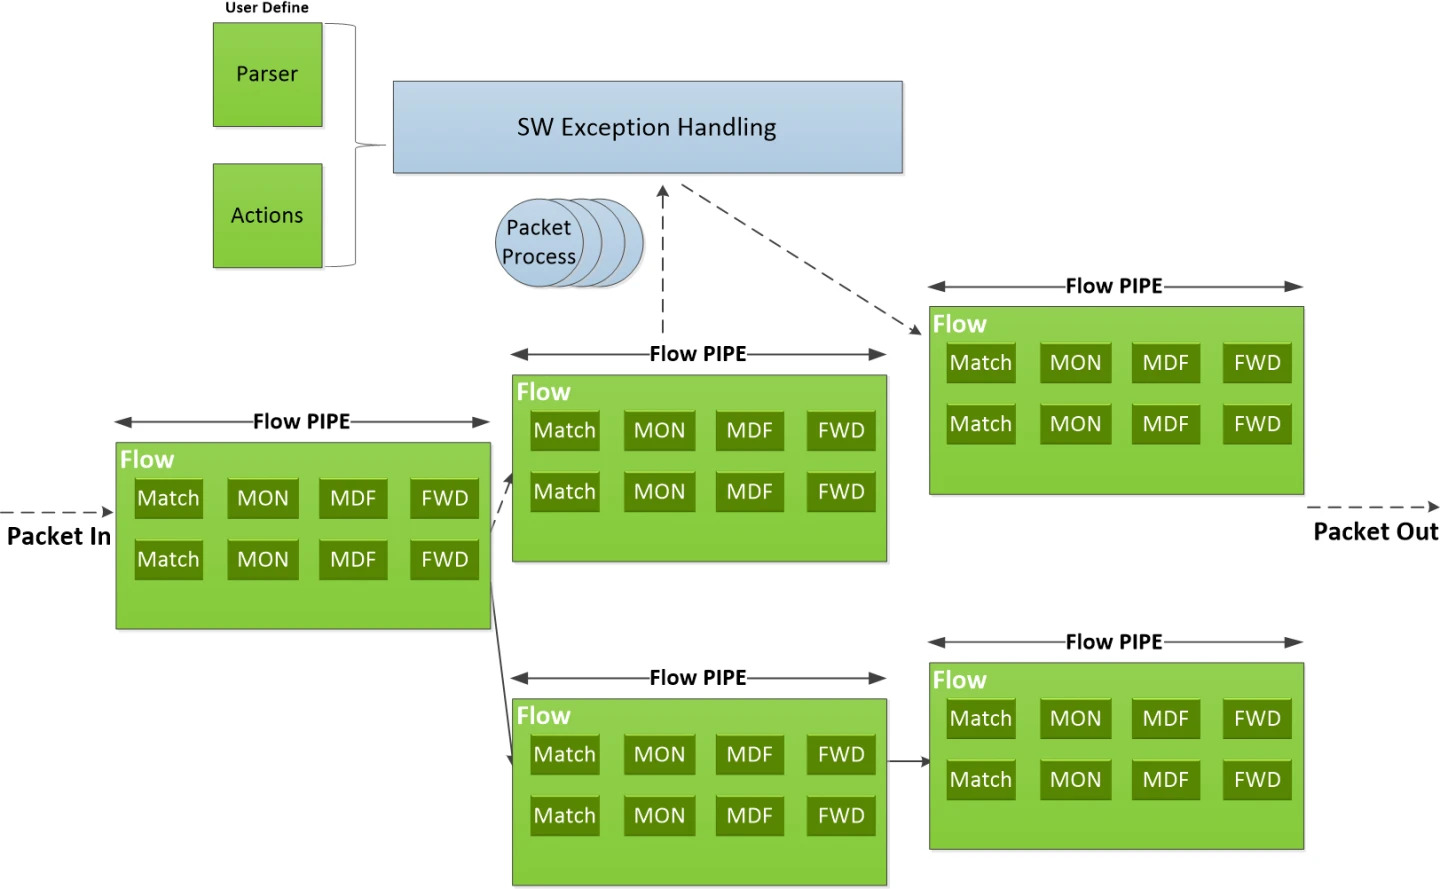
\includegraphics[width=1\linewidth]{img/docscontent.nvidia.jpg}
    \caption{Pipe Verschachtelung \cite{nvidia_doca_flow_architecture}}
    \label{fig:placeholder}
\end{figure}
Die zwei grundlegendsten Konzepte von DOCA Flows sind die der sogenannten \textbf{Pipes} und \textbf{Entries} \cite{nvidia_doca_flow_create_pipe_entry}. Diese beiden bilden zusammen den Kern der Funktionalität von DOCA Flow und erlauben neben den interessanten Paketmodifikationen (\textit{Actions}) auch weitere Features wie beispielsweise \textit{Matching}, \textit{Monitoring} und \textit{Forwarding}. Matching definiert zunächst anhand einer genauen Bitfelddefinition, welche Pakete explizit oder implizit aus dem Datenverkehr der Netzwerkkarte herausgenommen werden sollen und im weiteren Verlauf verarbeitet werden können. Das Monitoring erlaubt uns hierbei, ohne weiteren Overhead die Menge sowie die Größe des entsprechenden Netzwerkverkehrs zur Laufzeit beobachten zu können. Daraufhin werden die eigentlichen Actions ausgeführt, die es nun erlauben, Bitfelder auf L2, L3 und L4 des Pakets zu ändern. Abschließend wird mittels der Forwardingdefinition angegeben, an welches Ziel das verarbeitete Paket final weitergeleitet werden soll. Als Ziel können neben dem Hardware-Port auch Pipes oder sogar der ARM-Host angegeben werden. Die genannten Komponenten befinden sich allgemein in einer Pipe. Diese stellt eine Art Template dar, mit dem dann in den Entries die eigentlichen Implementierungen der genannten vier Bereiche zu finden sind. Entries werden einer entsprechenden Pipe zugeordnet und können nur solche Bitfelder beeinflussen, die als Template innerhalb der Pipe aktiviert wurden. Durch das Verketten von Pipes können hochkomplexe Anwendungen implementiert werden (siehe Abbildung 2.2).

\subsubsection{Hash-Pipes}
% Hash-Pipes ergänzen und Modi erklären
Hash-Pipes stellen einen besonderen Typ von Pipe dar. Sie erlauben die implizite Ausführung eines Hashing Algorithmus auf eingehende Pakete. Dieser Hashing Algorithmus erlaubt es dann, entsprechend dem Ergebnis der Anwendung einer Hashing Funktion Pakete auf den der Pipe zugeordneten Einträgen zu verteilen \cite{nvidia_doca_flow_pipe_hash}. Dabei ist es nicht möglich, den entsprechenden Hashing-Algorithmus zu bestimmen; vielmehr wird lediglich eine implementierung seitens Nvidia angeboten. Allerdings lassen sich gewisse Parameter anpassen, die es beispielsweise erlauben, alle Pakete an alle Entries zu senden oder die gewählten Bitfelder, die in den Hashing Algorithmus einfließen sollen, zu ignorieren und alle Pakete vollständig zufällig an alle Entries zu verteilen. Über welche Bitfelder gehashed werden soll, wird mittels der match Maske definiert. So kann beispielsweise entschieden werden, nur über den Source-Port zu hashen. 

Außerdem besitzen Hash-Pipes unterschiedliche Modi, die maßgeblich das Verhalten der Anwendung des Hashing-Algorithmus verändern.
\begin{itemize}
    \item \texttt{DOCA\_FLOW\_PIPE\_HASH\_MAP\_ALGORITHM\_HASH}: Dies ist der Standardalgorithmus, der implizit oder explizit bei der Erstellung der Hash-Pipe angegeben werden kann. Er verwendet eine nicht näher spezifizierte oder einsehbare Hash-Funktion zum bestimmen des Indexes der Pipe-Entries. 
    \item \texttt{DOCA\_FLOW\_PIPE\_HASH\_MAP\_ALGORITHM\_RANDOM}: Bei diesem Hash-Pipe-Modus werden Pakete zufällig auf die einer Pipe zugeordneten Entries verteilt.
    \item \texttt{DOCA\_FLOW\_PIPE\_HASH\_MAP\_ALGORITHM\_IDENTITY}: Das Identitätsbasierte Hashing verwendet eine Identitätsfunktion, die eine eins-zu-eins Beziehung zwischen einem Hashwert und dem entsprechenden Entry garantiert.
    \item \texttt{DOCA\_FLOW\_PIPE\_HASH\_MAP\_ALGORITHM\_FLOODING}: Der Flooding-Algorithmus dupliziert ein Paket und übergibt jedem erstellten Entry eine Kopie des Pakets. So kann garantiert werden, dass alle Entries eine Version des ursprünglichen Pakets erhalten.
    \item \texttt{DOCA\_FLOW\_PIPE\_HASH\_MAP\_ALGORITHM\_SELECT\_ENABLED}: Dieser Modus leitet alle Pakete zu einem bestimmten Entry weiter. Dabei kann nur ein einziges Entry als Target gewählt werden.
\end{itemize}
Die Verwendung einer solchen Hash-Pipe ermöglicht es Anwendungen, implizite Verteilungen auf die angelegten Entries einer Pipe auszuführen. Im Gegensatz dazu, also bei einer Basic-Pipe, müssten sonst alle entsprechenden Match-Regionen zur Laufzeit in jedem Entry explizit definiert werden. Dies würde sicherlich mit einem erheblichen Implementierungsaufwand einhergehen.
\subsection{Hardware Beschleuniger}
%hier auf eSwitch, DPL-Parser, DPL-MatchAction eingehen
Der für diese Arbeit wohl wichtigste Hardware-Beschleuniger ist der zuvor genannte eSwitch. Dieser setzt sich im wesentlichen aus drei Komponenten zusammen. Grundsätzlich wird der eSwitch mithilfe einer P4-abgewandelten Sprache namens DOCA Pipelining Language (DPL) programmiert. Die DPL beschreibt wiederum das Verhalten der drei Hauptbestandteile des eSwitches. Zunächst einmal treffen Pakete beim \textbf{DPL-Parser} ein. Dieser bricht das zunächst serielle Paket in eine Bitfeldrepräsentation auf und ermöglicht so die schnellen und Effizienten Bitwise Operationen innerhalb der ASICs. Daraufhin werden die Pakete an die \textbf{DPL-Tabelle} weitergeleitet. Diese enthält die Kombination eines Matches und einer entsprechenden Action und ist somit die Kernausführungs-Einheit im eSwitch. Schließlich werden die Pakete entsprechend den Einträgen in der \textbf{Forwarding-Datenbank} an das entsprechende Ziel weitergeleitet. Der Zusammenhang dieser drei Einheiten ist ebenfalls in Abbildung 2.1 zu sehen.
\section{XenoFlow 0.1 aus der Bachelorarbeit}
\textit{Dieses Projekt ist als Anschluss an die Ursprüngliche Implementierung eines Loadbalancers zu verstehen, den ich im Rahmen meiner Bachelorarbeit im ersten Quartal 2025 implementiert habe. Zum damaligen Zeitpunkt war es aufgrund des Umfangs der Thematik nicht möglich, auf architektonische Details einzugehen, was allerdings nun in diesem Rahmen passieren soll.}
\subsection{Was bisher geschah...}
% Professioneller Ton
\begin{figure}
    \centering
    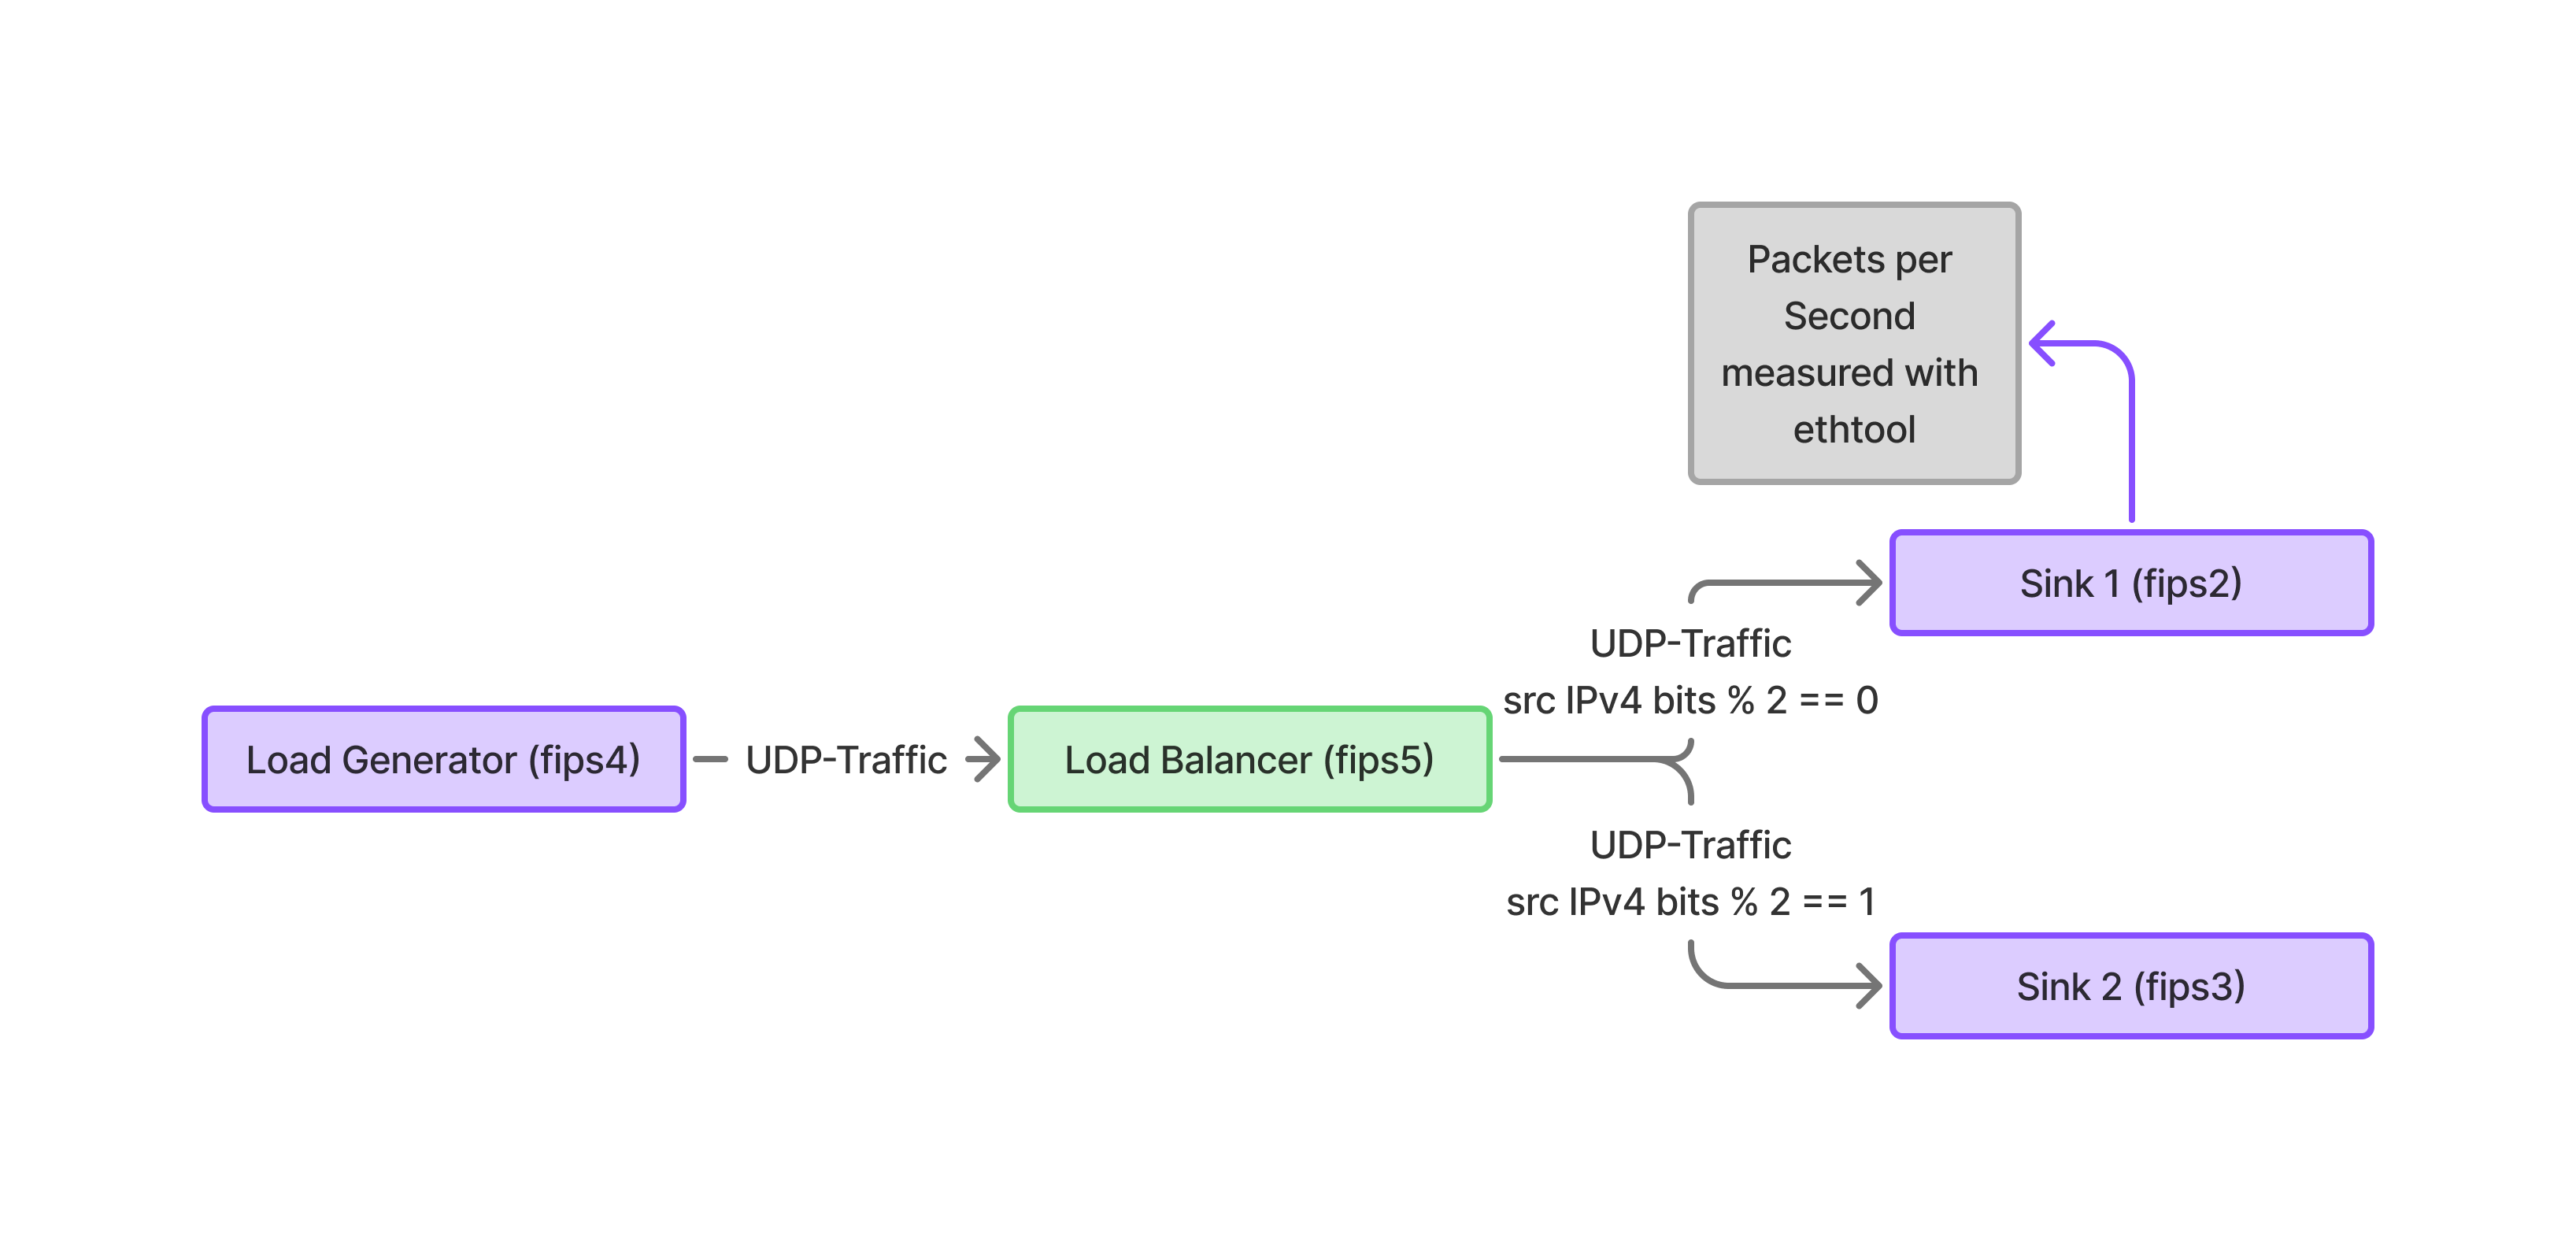
\includegraphics[width=1\linewidth]{img/Messaufbau PPS.png}
    \caption{Prototyp XenoFlow mit zwei Backends \cite{heimbrodt2025xenoflow}}
    \label{fig:placeholder}
\end{figure}
XenoFlow war in seiner ursprünglichen 0.1 Fassung ein L3-Loadbalancer, der anhand der Source-IP-Adresse mithilfe eines selbst implementierten, bitfeldbasierten Pseudohashings die Lastverteilungsentscheidung getroffen hat. Dabei wurden je nach Anzahl der aktiven, ansprechbaren Backends die letzten Bits der Source-IP-Adresse als Matchkriterium für die Entries verwendet, die daraufhin schließlich an das entsprechende Backend mittels eines Des-tination-MAC-Adressen-Rewrites weitergeleitet wurden. Das gesamte Projekt wurde damals mittels DOCA Flow implementiert. Grundsätzlich war der Loadbalancer allerdings sehr statisch. Es wurde zu Programmstart einmal aus einer Config-YAML-Datei die aktuelle Konfiguration ausgelesen und entsprechend installiert. Es war also insbesondere keine Änderung der Backends zur Laufzeit möglich. Außerdem hatte der pseudo Hashingalgorithmus das Problem, dass er anfällig für Strukturen in IP-Adressen war, da ein Filtern keiner direkten Hashfunktion entspricht. Dies gilt vor allem, da nur wenige Bits der Source-IP zur Aufteilung verwendet wurden. Es musste also davon ausgegangen werden, dass die letzten Bits der Source-IP-Adresse ausreichend hoch entropisch sind, um äquivalent große Klassen von Paketen für die Lastverteilung zu erzeugen. Diese Funktionsweise ist in Abbildung 3.1 dargestellt.
\subsection{Ergebnisse}
\begin{figure}
    \centering
    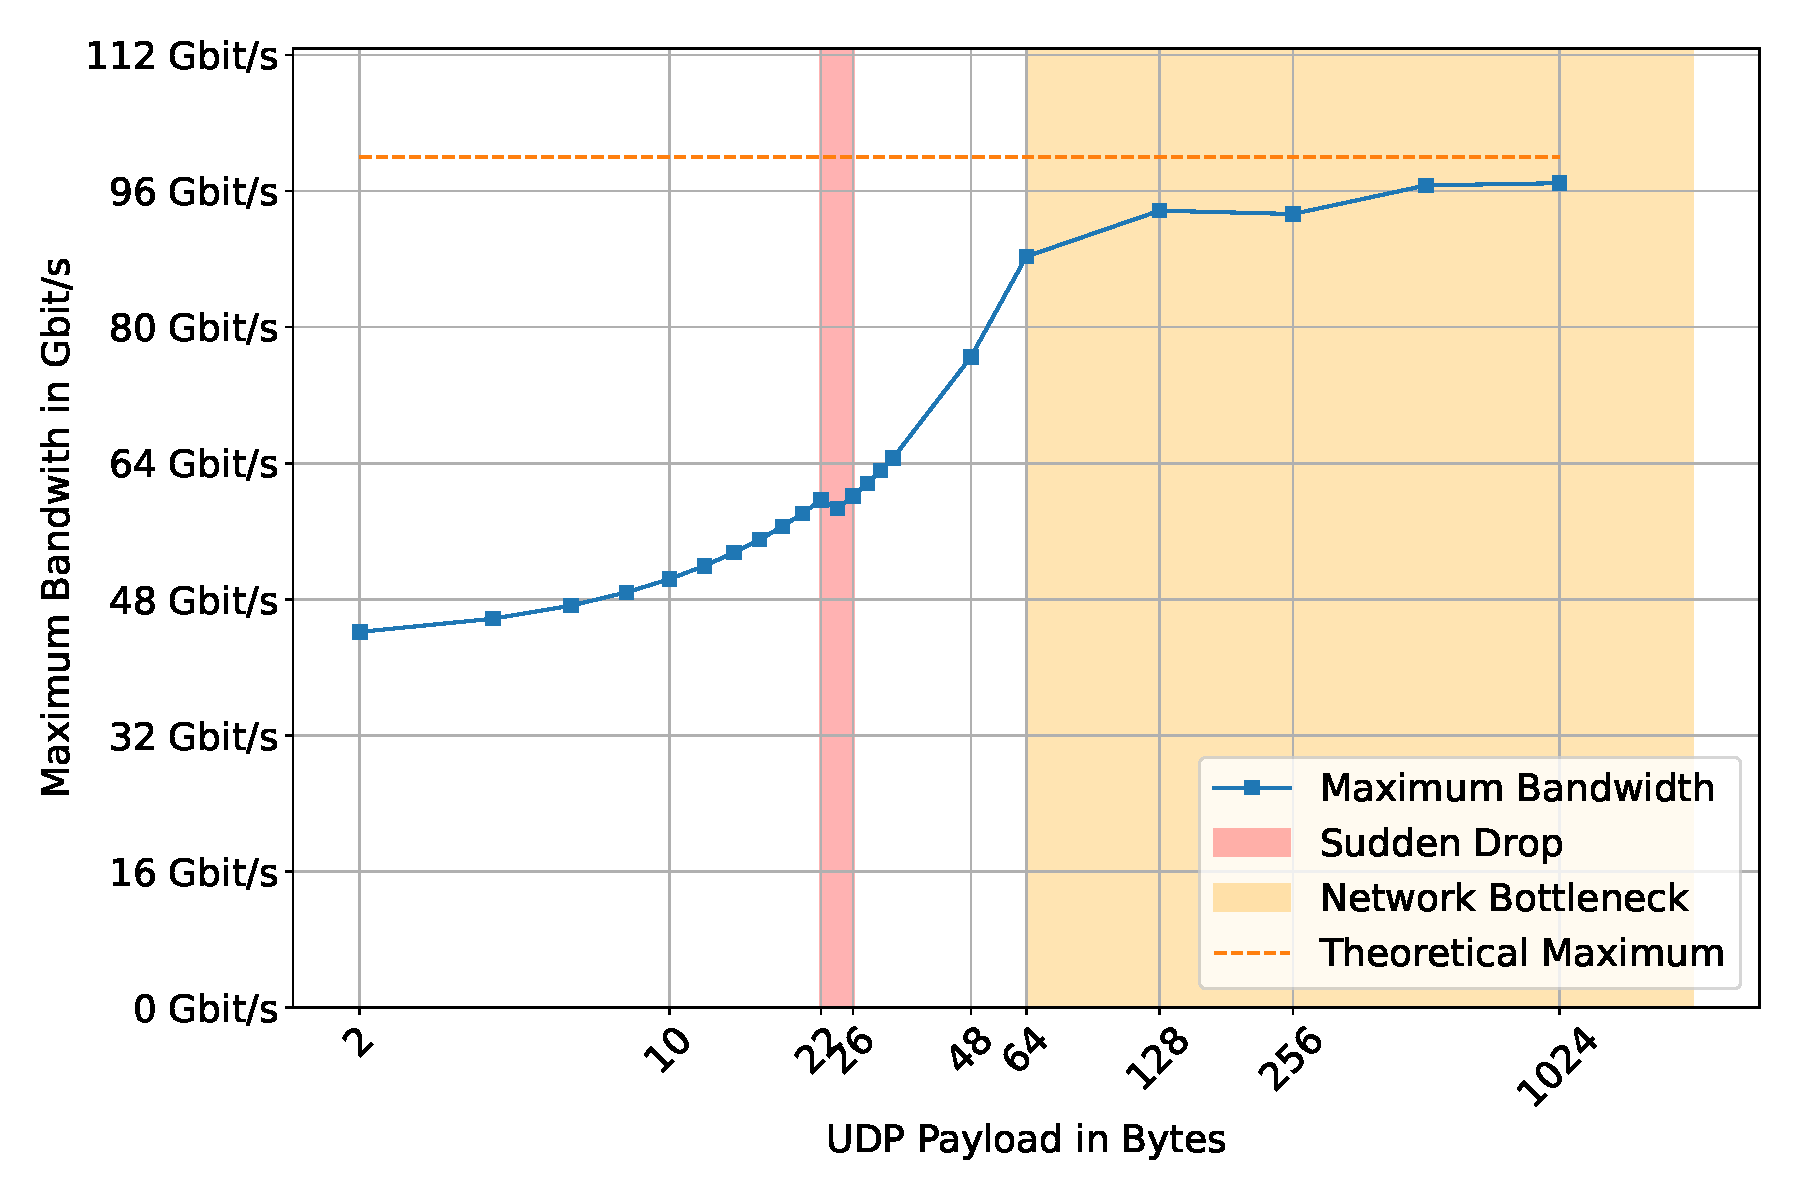
\includegraphics[width=1\linewidth]{img/pps_bandwidth.pdf}
    \caption{Pakete pro Sekunde - Bandbreite \cite{schroetter2026xenoflow}}
    \label{fig:placeholder}
\end{figure}
\begin{figure}
    \centering
    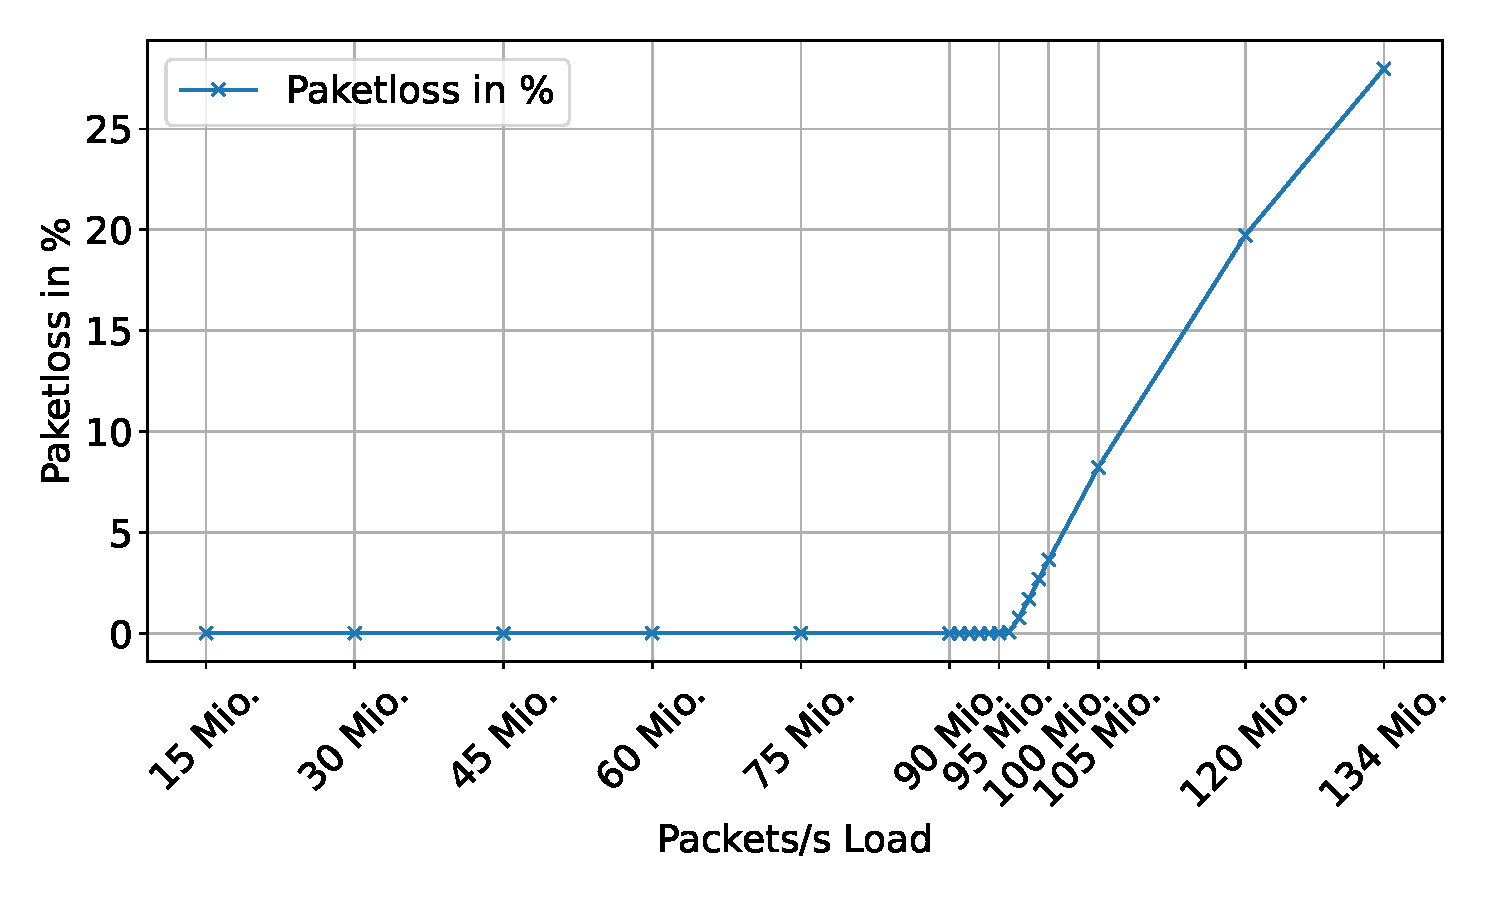
\includegraphics[width=1\linewidth]{img/pps_paketloss.pdf}
    \caption{Verlorene Pakete pro Sekunde in Prozent \cite{schroetter2026xenoflow}}
    \label{fig:placeholder}
\end{figure}
Wie in Abbildung 3.2 zu erkennen ist, war es möglich, eine Last von ca. 100 Gbit/s zu verarbeiten. Allerdings war dies nur bei einer Paketgröße von 128 Bytes möglich. Bei kleineren Paketen stellte sich als absolute Grenze der Verarbeitungsgeschwindigkeit in Paketen pro Sekunde 98 Millionen Pakete pro Sekunde bei einer Größe von weniger als 64 Byte und analog 95 Millionen Pakete pro Sekunde bei einer Größe von mehr als 64 Byte heraus. Diese abrupte Änderung ist in Abbildung 3.2 als \textit{Sudden Drop} betitelt. Wird der Schwellwert überschritten, so werden alle weiteren Pakete, wie in Abbildung 3.3 zu erkennen ist, gedroppt. Die Pakete kommen also noch auf dem Hardwareport der SmartNIC an, werden aber nicht mehr von der Verarbeitungspipeline erfasst und gehen an unbekannter Stelle verloren. Der Anstieg des entstehenden Paketverlusts ist fast linear, und es lässt sich somit davon ausgehen, dass das begrenzende Bottleneck die Taktung eines der verarbeitenden ASICs oder FPGAs ist. Zudem wurden Experimente zum Einfluss der Verarbeitung auf die Round-Trip-Time-Latenz durchgeführt, die gezeigt haben, dass es keinen messbaren Einfluss auf die Verarbeitungsgeschwindigkeit und Bandbreite gab. Dies war insbesondere auch unabhängig von der auf die Netzwerkkarten einwirkenden Last, da zusätzlich zu den Messpaketen auch eine künstliche Basislast erzeugt wurde, die ebenfalls auf den Loadbalancer gerichtet war.
\newpage
\section{Experimente}
Im folgenden werden nun die Konkreten Experimente beschrieben, anhand derer die Kennzahlen der BlueField ermittelt werden sollen. Ziel ist es, implizite und unbekannte Grenzwerte der Hardware zu ermitteln. Hintergrund ist es, eine Basis zu schaffen, auf der Entscheidungen hinsichtlich einer möglichen Implementierung von Anwendungen getroffen werden können. So kann beispielsweise die maximal mögliche Durchsatzrate zwischen zwei Hardwareports extrem relevant dafür sein, wo genau in der Topologie die BlueField eingesetzt wird. Alle folgenden Experimente wurden auf dem FIPS-Cluster des Lehrstuhls \textit{Betriebssysteme und Rechnernetze} von Prof. Dr. Bettina Schnor ausgeführt. Die Testumgebung wurde wie folgt aufgesetzt:
\begin{itemize}
    \item fips1 - Startknoten für besondere Pakete \textit{Intel Xeon Silver 4314, 128 GB RAM}
    \item fips2 - Endknoten (Sink) mit Paket-Timestamperfassung \textit{Intel Xeon Silver 4314, 128 GB RAM}
    \item fips3 - Endknoten (Sink) \textit{Intel Xeon Silver 4314, 128 GB RAM}
    \item fips4 - Lastgenerator mittels T-Rex \textit{Intel Xeon Silver 4314, 128 GB RAM}
    \item fips5 - Messknoten mit BlueField-3 NIC \textit{Intel Xeon Silver 4514Y, 128 GB RAM, ARM Cortex A78, 32 GB RAM}
\end{itemize}

\subsection{ebpf\_mac\_rewrite}
Die Motivation dieses Experiments besteht darin, einen sinnvollen Vergleichswert zu den gemessenen Bandbreiten der BlueField-3 zu bestimmen und die Hardware-Beschleunigung direkt mit einer traditionell auf der CPU ausgeführten Variante vergleichen zu können. Dazu wurde das aktuelle Framework der eBPF Implementierung des Linux-Kernels gewählt. 

eBPF ermöglicht es, eigenständig implementierte Funktionen an Events aus dem Kernelspace zu hängen und somit asynchron auf Signale aus dem Kernel reagieren zu können. Dieses Vorgehen erlaubt es, extrem effizient und Latenzarm auf ein Ereignis zu reagieren, da die Anwendungen tatsächlich im Kernelspace ausgeführt werden können. Dabei wird das Express Data Path (XDP) aus eBPF verwendet \cite{vieira2020ebpfxdp}. XDP erlaubt es, große Teile des Linux Netzwerkstacks zu umgehen und direkt in der Anwendung zu verarbeiten. Dies dient abermals der Effizienzsteigerung und Latenzverringerung. In Listing 1 wird ein eBPF Programm beschrieben, welches die Ziel-MAC-Adresse eines eingehenden Pakets ändert. Damit soll die Action des XenoFlow Loadbalancers simuliert werden, die die tatsächliche Änderung der Ziel-MAC vornimmt. Dazu sei erwähnt, dass das entsprechende Matching, also die Auswahl des Pakets aus dem Datenstrom, hier nicht implementiert wird. Der Vergleich ist somit ein best-case im Vergleich zu XenoFlow, da wesentlich weniger Overhead aufkommt. Zusätzlich wurde im gleichen Stil ein weiteres Programm für die ConnectX-7 implementiert, um den genannten Matching Overhead auszuschließen. Bei besagtem Programm wird ebenfalls lediglich die Ziel-MAC-Adresse, ohne Matching, geändert. Da ConnectX-7 ebenfalls mittels DOCA Flow programmiert werden kann, war der Code-Aufwand dafür relativ gering, und es konnten weite Teile von XenoFlows Kern nachverwendet werden. Grundsätzlich wird in diesem Experiment die Laufzeit zwischen dem Senden eines Pakets von fips1 über den entsprechenden Action Host (also entweder BlueField oder eBPF Host) weitergeleitet zu einem Backend. Wird der Sende-Zeitstempel von dem Empfangs-Zeitstempel abgezogen, so bildet dies die Round-Trip-Time.
\label{code:ebpf-code}
% Mehr auf konkrete Codezeilen eingehen (erklären)
% Intrinsic-Signatur
\begin{minted}[linenos]{c}
SEC("xdp")
int xdp_mac_rewrite(struct xdp_md *ctx)
{
    void *data     = (void *)(long)ctx->data;
    void *data_end = (void *)(long)ctx->data_end;

    /* ... */

    __be32 fips1 =0x04030201;

    if ( __builtin_memcmp(&ip->saddr, &fips1, 4)) 
        return XDP_PASS;

    struct mac_addr key = {};
    __builtin_memcpy(key.addr, eth->h_source, ETH_ALEN);

    const struct mac_addr *new_dst = bpf_map_lookup_elem(&mac_redirect_map, &key);

    __builtin_memcpy(eth->h_dest, new_dst->addr, ETH_ALEN);
    // New source MAC: a6:03:ff:17:2b:3a
    eth->h_source[0] = 0xA6;
    eth->h_source[1] = 0x03;
    eth->h_source[2] = 0xFF;
    eth->h_source[3] = 0x17;
    eth->h_source[4] = 0x2B;
    eth->h_source[5] = 0x3A;

    return XDP_TX;
}
\end{minted}
Das Code-Stück zeigt die an ein Paket-Empfang geknüpfte Call-Back-Funktion, die die entsprechenden MAC-Header-Felder ändert. Zunächst wird in Zeile 9 die Source-IP definiert, die durch ein Match zwischen dem eingehenden Paket und dem eigenen Wert zur weiteren Paketverarbeitung führen soll. Alle anderen Source-IPs sollen regulär weitergegeben werden. Der eigentliche Vergleich zwischen der Variablen \texttt{fips1} und der \texttt{saddr} findet mittels der \texttt{\_\_builtin\_memcmp()} in Zeile 11 statt. Alle Pakete, die nicht der entsprechenden \texttt{fips1}-IP entsprechen, geben bei diesem eBPF Funktionsaufruf also \texttt{XDP\_PASS} zurück und werden regulär weitergeleitet. Das Umschreiben der Ziel-MAC-Adresse findet zuletzt in Zeile 19 bis 26 statt, in denen die Memory Region durch die neu erstellte \texttt{new\_dst}-Adresse ersetzt wird und die entsprechenden MAC-Adressen-Teile für den neuen Zielknoten eingetragen werden.
\subsubsection*{Ergebnisse}
\label{experiment:rtt}
\begin{figure}
    \centering
    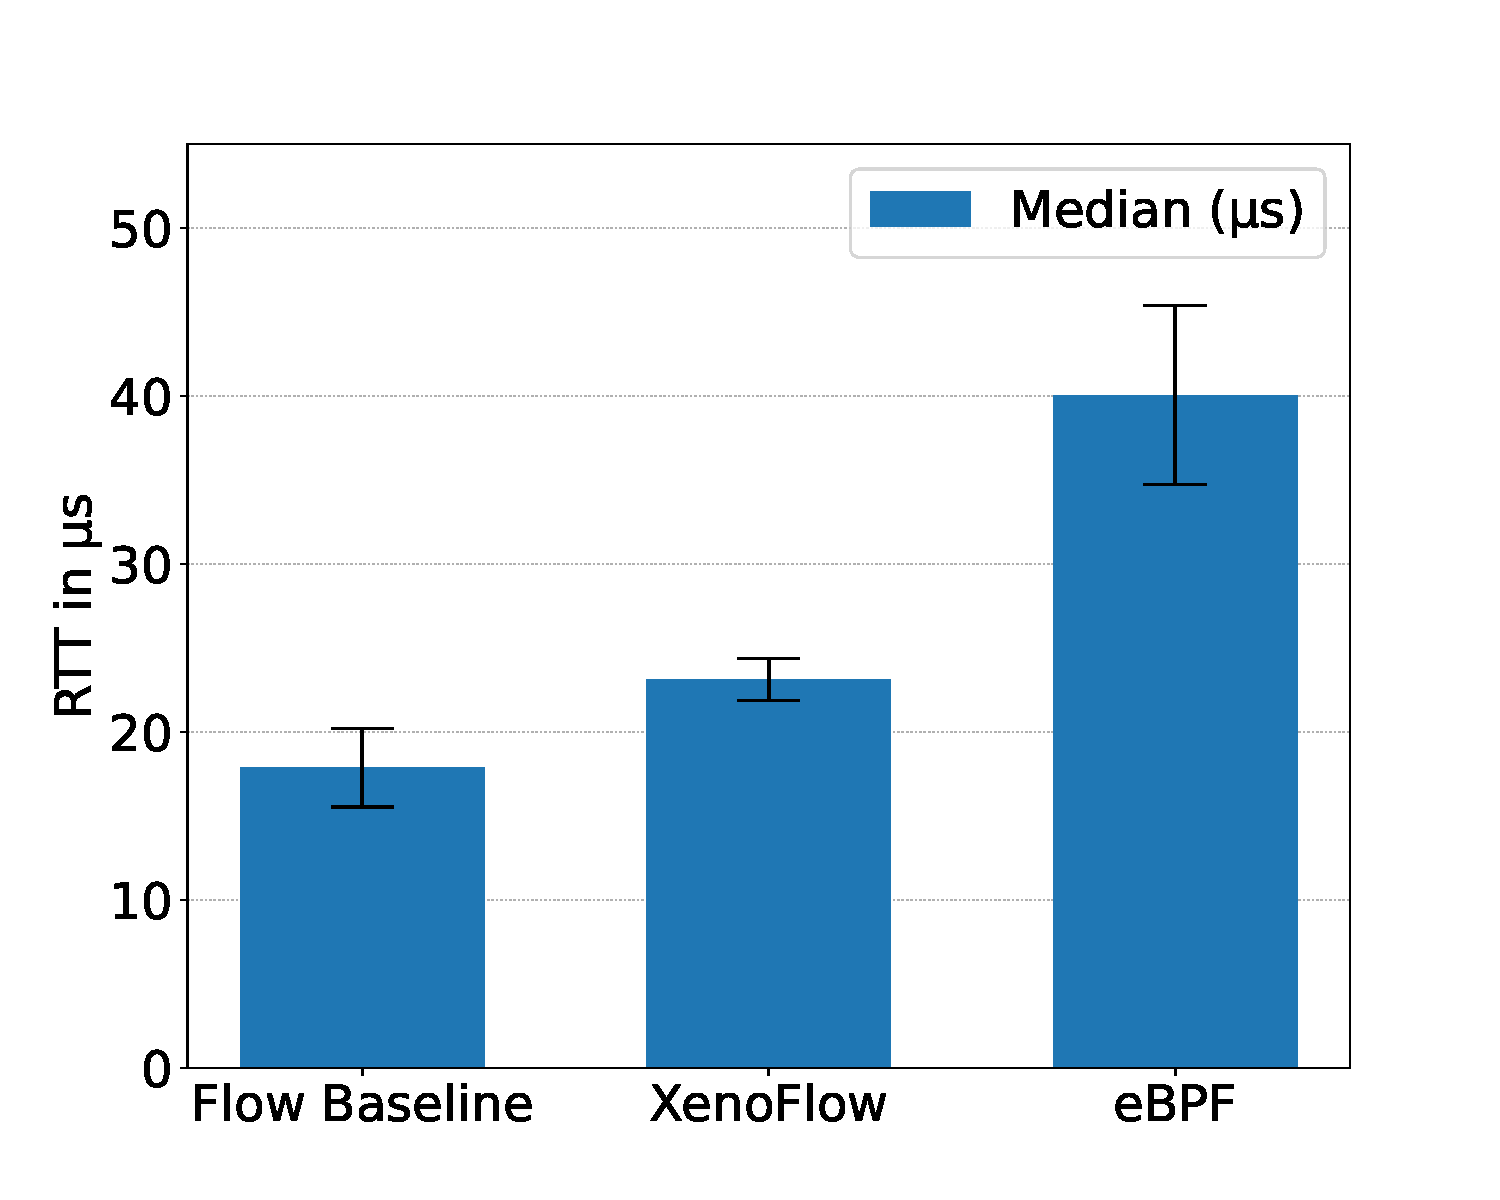
\includegraphics[width=1\linewidth]{img/rtt.pdf}
    \caption{Round-Trip-Time Vergleich \cite{schroetter2026xenoflow}}
    \label{fig:placeholder}
\end{figure}
% Auf Flow baseline eingehen und ggf. erweitern
Wie in Abbildung 4.1 zu sehen ist, ist die RTT eines vergleichbaren eBPF-Programms \textbf{wesentlich größer} als die von XenoFlow. Außerdem ist zu beachten, dass das verwenden eines Matches ebenfalls mit signifikanten Leistungseinbußen einhergeht, da die Flow Baseline noch besser performt als der XenoFlow Loadbalancer. Dies kann angenommen werden, da der einzige Unterschied zwischen der \texttt{Flow Baseline} und der \texttt{XenoFlow} in diesem Experiment der zusätzliche Match ist, der bei \texttt{XenoFlow} zum Verteilen der Last verwendet wird. Alle drei Implementierungen führen im Kern allerdings dieselbe Operation durch und ändern nach dem Erhalt eines Paketes mit einer bestimmten Source-IP die Target-MAC auf den empfangenden Messknoten.
\subsection{max\_pipes}
Im max\_pipes Experiment wird untersucht, wie viele Pipes in DOCA Flow von einer Anwendung aus angelegt werden können. Da eine Pipe ein Template darstellt, kann man davon ausgehen, dass die gemessene Anzahl maximaler Pipes pro Anwendung aussagt, wie viele unterscheidbare Templates der zugrunde liegenden Templating-Engine angelegt werden können. Im folgenden Code wird versucht, unbegrenzt viele Pipes anzulegen. Ziel ist es herauszufinden, wann die Laufzeit abstürzt und ob das Ergebnis reproduzierbar ist. 


% Diff zur Nvidia Docu aufzeigen
\begin{minted}[linenos]{c}
while(1) {
    create_root_pipe(ports[0], 0, DOCA_FLOW_L4_TYPE_EXT_UDP, &udp_pipe);

    DOCA_LOG_INFO("Added nr %i", nr_pipe);
    nr_pipe++;
}
\end{minted}
In diesem Code-Ausschnitt wird die eigens definierte Funktion \texttt{create\_root\_pipe()} aufgerufen, welche wiederum die DOCA-Flow-intrinsische Funktion \texttt{doca\_flow\_pipe\_create()} aufruft.
\begin{minted}[linenos]{c}
doca_error_t doca_flow_pipe_create_v1(
    const struct doca_flow_pipe_cfg * cfg, 
    const struct doca_flow_fwd_v1 * fwd, 
    const struct doca_flow_fwd_v1 * fwd_miss, 
    struct doca_flow_pipe ** pipe
);
\end{minted}
Die \texttt{doca\_flow\_pipe\_cfg} gibt hier die entsprechenden Feldaktivierungen an. Diese beschreiben, welche Felder im folgenden von Entries verwendet werden können, um entweder Matching oder Actions zu erlauben. Aber auch IDs für den späteren Monitoring Zugriff müssen hierin bereits mittels einer Maske angelegt werden. Mehr dazu in der DOCA Flow Dokumentation unter \url{https://networking-docs.nvidia.com/doca/archive/3-4-0/doca-flow}. Die beiden Unterstrukturen \texttt{doca\_flow\_fwd\_v1 fwd} und \texttt{fwd\_miss} geben an, an welches Ziel bei einem entsprechenden Hit oder Miss einer Pipe weitergeleitet werden soll. Zuletzt wird die vom Nutzer angelegte Datenstruktur \texttt{struct doca\_flow\_pipe ** pipe} per Referenz übergeben, damit DOCA Flow das entsprechende Struct mit Werten füllen kann.
\subsubsection*{Ergebnisse}
Ab einer Anzahl von \textbf{505} Pipes endet die DOCA Flow-Laufzeit mit einem Fehlercode 0. Es ließ sich leider keine Bedeutung aus der DOCA Flow Dokumentation finden. Das Experiment wurde dreimal durchgeführt, und das Ergebnis konnte jedes mal reproduziert werden.
\newpage
\subsection{max\_entries}
Im max\_entries Experiment wurde sehr ähnlich zum max\_pipes Experiment einfach so lange das entsprechende Entry erzeugt, bis es zu einem Laufzeitfehler kam. Es wurden die Entries zu einer einzigen Pipe hinzugefügt, sodass der ermittelte Wert als maximale Anzahl an Entries pro Pipe angesehen werden kann. Zusätzlich müssen die hinzugefügten Entries noch verarbeitet werden. Dies geschieht ebenfalls mit einer intrinsischen Funktion, wie im folgenden Code zu sehen ist:
\begin{minted}[linenos]{c}
while(1) {
    result = doca_flow_pipe_add_entry(
        0, udp_pipe, &match, &actions, &monitor, 
        DOCA_FLOW_NO_WAIT, 0, &status, &entry
    );
    result = doca_flow_entries_process(
        ports[0], 0, DEFAULT_TIMEOUT_US, 
        num_of_entries
    );
    nr_entry += 1;
    DOCA_LOG_INFO("Added nr %i", nr_entry);
}
\end{minted}
Die beiden wichtigen DOCA-Funktionen sind hier nun \texttt{doca\_flow\_pipe\_add\_entry()} und \texttt{doca\_flow\_entries\_process()}.
\begin{minted}[linenos]{c}
doca_error_t doca_flow_pipe_basic_add_entry_v1(
    uint16_t pipe_queue, 
    struct doca_flow_pipe * pipe, 
    const struct doca_flow_match_v1 * match, 
    uint8_t action_idx, 
    const struct doca_flow_actions_v1 * actions, 
    const struct doca_flow_monitor_v1 * mon, 
    const struct doca_flow_fwd_v1 * fwd, 
    uint32_t flags, 
    void* usr_ctx, 
    struct doca_flow_pipe_entry** entry
);
\end{minted}
Mittels dieser Funktion können Entries einer Pipe zugeordnet werden. Die entsprechende Pipe wird als Pointer übergeben. Dort sind wieder die bekannten Datenstrukturen Match, Actions, Monitor und Forward aus der Pipe-Definition zu erkennen. Leider konnte zur genauen Bedeutung der restlichen Felder keine Erklärung gefunden werden. Wir erhalten lediglich den entsprechenden Header unter \texttt{/opt/mellanox/doca/include/doca\_ctsd\_flow.h}, und die zugehörigen Implementierungen befinden sich in kompilierten Shared-Objects. 
\newpage
Nach dem Hinzufügen eines Entries sind diese allerdings noch nicht aktiv. Dies passiert erst nach dem Aufruf der folgenden Funktion:
\begin{minted}[linenos]{c}
doca_error_t doca_flow_entries_process(
    struct doca_flow_port *port,
    uint16_t pipe_queue,
    uint64_t timeout,
    uint32_t max_processed_entries
);
\end{minted}
Hierbei werden neben dem Port (Zeile 2) auch der Timeout angegeben, indem das Entry eingetragen werden muss (Zeile 4). Worauf sich die \texttt{pipe\_queue} bezieht, ist aus dem Header \texttt{/opt/mellanox/doca/include/doca\_flow.h} leider nicht ersichtlich. Dort wird lediglich \textit{Queue identifier} als Funktions-Parameter-Dokumentation angegeben. 
\subsubsection*{Ergebnisse}
Nach einer Anzahl von \textbf{8192} Einträgen in einer Pipe beendet die DOCA Flow runtime mit einem Fehler. Dazu sei erwähnt, dass die Runtime bereits nach dem hinzufügen abstürzt, also insbesondere vor dem eigentlichen Prozessierungsaufruf. In neueren DOCA Flow Versionen ist es nun allerdings auch möglich, die Größe der Pipes anzupassen und entsprechend mehr Entries hinzuzufügen.

\newpage

\subsection{PCC}
% Genauer auf Skript eingehen
Eine der wichtigsten Anforderungen für einen Loadbalancer wie XenoFlow, der auf L3 agiert, ist es, die Konsistenz des Kontexts der Backends für TCP-Verbindungen zu wahren. TCP Verbindungen sind stateful und ermöglichen es, zwischen Client und Server einen Kontext zu etablieren, der komplexere Anwendungen ermöglicht. Dies ist für einen Loadbalancer dringend zu beachten, da sonst zwei Pakete desselben Kontextes an unterschiedliche Backends weitergeleitet werden. Somit wäre die Konsistenz gebrochen und die Kontextsicherheit zerstört. Daher ist es notwendig, sicherzustellen, ob Hash Pipes wirklich nur auf den angegebenen Feldern den Hashing Algorithmus anwenden oder auch implizit andere Felder wie timestamps oder ähnliches mit einbeziehen, die die Hash Funktion negativ beeinflussen würden. Um dies zu testen, wurde ein Python Skript entwickelt, welches bestimmte Felder variiert und zeigt, wie sich das Hashing verhält.
\begin{minted}[linenos]{python}
# ...
if __name__ == "__main__":
    print("=== Test 1: Variierende Portnummern ===")
    for i in range(8000, 8500, 1):
        send_udp_packet(
            dest_port=i, payload=f"Hello {i}", interface="enp24s0f0np0"
        )
    print("\n=== Test 2: Variierende Src-IPs ===")
    for i in range(1000):
        src_ip = f"10.2.{i // 256}.{i % 256}"
        send_udp_packet_with_src_ip(
            src_ip=src_ip, dest_port=80, 
            payload=f"From {src_ip}", interface="enp24s0f0np0"
        )
    print("\n=== Test 3: Variierende Dst-IPs ===")
    for i in range(500):
        dst_ip = f"10.0.{i // 256}.{i % 256}"
        send_udp_packet_with_dst_ip(
            dst_ip=dst_ip, dest_port=80, 
            payload=f"To {dst_ip}", interface="enp24s0f0np0"
        )
\end{minted}
In diesem Python Skript werden 3 Tests durchgeführt.
\begin{itemize}
    \item Test 1: Variiert die Destination-Port-Nummer und sendet UDP-Pakete.
    \item Test 2: Variiert die Source-IP und sendet UDP-Pakete.
    \item Test 3: Variiert die Destination-IP und sendet UDP-Pakete.
\end{itemize}
\subsubsection*{Ergebnisse}
Es konnte gezeigt werden, dass in der Tat lediglich die per Match-Definition bestimmten Bitfelder in die Hash Berechnung einfließen. Das bedeutet, dass zwei Pakete mit entsprechend gleicher Signatur garantiert beim gleichen Backend landen werden. Diese Tatsache legt eine wichtige Grundlage für die spätere Implementierung fest, da dieser Fakt benötigt wird, um die Bucket Semantik abbilden zu können. Nur mit der Gewissheit einer persistenten Hashing-Zuordnung kann gewährleistet werden, dass kontextbehaftete Protokolle wie beispielsweise TCP unterstützt werden.
\subsection{entry\_latency}
% PTP Setup genauer beschreiben
Die aufwendigste Untersuchung und somit auch das komplexeste Experiment dieser Projektarbeit beschäftigt sich mit der Latenz des Einfügens eines Eintrags in eine Pipe. Dabei soll gemessen werden, wie viel Zeit zwischen dem Funktionsaufruf zum Hinzufügen eines Elements und dem tatsächlichen Aktivwerden vergeht. Damit die gemessenen Latenzwerte nah an einer realistischen Umgebung sind, wurde das ganze als eine verteilte Messung über insgesamt drei Knoten durchgeführt. 

Grundsätzlich war die Idee, auf einem Knoten (fips1) einen kontinuierlichen Paketstrom zu erzeugen. Auf der BlueField-3 wurde auf der Seite des ARM-Hosts während dieses Paketstroms ein Entry erzeugt und einer Pipe hinzugefügt. Dabei wird ein Erstellungs-Zeitstempel erfasst. Sobald nun diese Entry-Regel aktiv ist, werden Pakete an den dritten Host (fips3) weitergeleitet. Dort wird beim Empfangen des ersten Pakets ebenfalls der Zeitstempel als Empfangs-Zeitstempel erfasst. Die Idee ist es nun, den Erstellungs-Zeitstempel vom Empfangs-Zeitstempel abzuziehen. Der erhaltene Wert gibt dann die Zeit an, in der die DOCA Flow Laufzeit die entsprechende Erstellung und Aktivierung vornimmt. Dazu sei erwähnt, dass natürlich die Netzwerklatenz abgezogen werden muss, um die tatsächliche Hardware-Laufzeit zu bestimmen. Das Problem ist nun, dass die Messung im Bereich von $\mu$-Sekunden stattfindet. Somit ist es zwingend erforderlich, dass die beiden zeitnehmenden Knoten ihre Uhren synchronisieren. 

Als Basisuhr wurden die Hardware-Uhren der jeweiligen Netzwerkkarten genutzt. Die beiden Hosts wurden untereinander mittels \textbf{PTP} synchronisiert. Damit die Hardware-Uhren der Netzwerkkarte auch im Kernel verfügbar sind, wurde das Tool \texttt{phc2sys} aus dem Linux-PTP-Paket verwendet. Das Tool erlaubt es, zwischen der Netzwerkkarte und dem Linux-Kernel sehr genau zu synchronisieren. Dies wurde sowohl auf der BlueField-3 selbst als auch auf dem empfangenden Knoten durchgeführt.

Beim Synchronisieren war die Hardware-Uhr der BlueField-3 sehr auffällig ungenau und hatte einen Jitter mit einer maximalen Auslenkung von $24 \mu s$ (Synchronisation zwischen Con-nectX-7-Karte und Bluefield-3 Hardware-Clock). Dies ist eigentlich sehr ungewöhnlich, da Netzwerkkarten-Hardware-Uhren normalerweise gegen einen Kristalloszillator synchronisieren, der eine Genauigkeit im $ns$-Sekundenbereich hat. 

Ein weiteres großes Problem war, dass es normalerweise notwendig ist, eine hohe Paketfrequenz zu verwenden, um die Genauigkeit der Messung zu erhöhen. Da allerdings auf dem fips3 Backend mittels eines klassischen Tcpdumps gemessen wurde, musste eine andere Herangehensweise entwickelt werden, um zu vermeiden, dass die entsprechenden Log-Dateien extrem groß werden. Dazu wurde eine gemäßigtere Anzahl an Paketen pro Sekunde verschickt, die allerdings mit einer Zufälligen Wartezeit zwischen den Paketen abgeschickt wurden. Durch dieses künstliche Streuen der Sende-Zeitstempel ist es möglich, statistisch an die tatsächlichen Werte des ersten Empfangs zu kommen. Im folgenden Code ist der random delay zu sehen:
\begin{minted}[linenos]{c}
while(1) {
    struct timespec ts;
    int random_delay = (rand() % 10000) + 1;
    /*...*/
    DOCA_LOG_INFO(
        "Adding entry at: %02d:%02d:%02d.%09ld", 
        tm.tm_hour, tm.tm_min, tm.tm_sec, ts.tv_nsec
    );

    doca_flow_pipe_add_entry(/* Entry Parameter */);
    doca_flow_entries_process(/* Entry Process Parameter */);

    usleep(statRefreshIntervall + random_delay);

    DOCA_LOG_INFO(
        "Removing entry at: %02d:%02d:%02d.%09ld", 
        tm.tm_hour, tm.tm_min, tm.tm_sec, ts.tv_nsec
    );
    
    doca_flow_pipe_remove_entry(/* Entry Remove Parameter */);
    doca_flow_entries_process(/* Entry Process Parameter */);
}
\end{minted}
In Zeile 3 wird eine zufällige Backoff-Zeit errechnet, die, wie vorher beschrieben, die Messung mit deutlich niedrigeren Datenraten ermöglicht und anschließend in Zeile 13 angewendet wird. Ansonsten kommt das Experiment mit den hier zuvor eingeführten Funktionen aus.  \begin{minted}[linenos]{c}
doca_error_t doca_flow_pipe_remove_entry(
    uint16_t pipe_queue, 
    uint32_t flags, 
    struct doca_flow_pipe_entry *entry
);
\end{minted}
Die \texttt{doca\_flow\_remove\_entry()} ist allerdings neu und erlaubt unter der Angabe der Pipe-Queue und des Entry, analog zum Hinzufügen, auch das Löschen eines Entries aus einer Pipe.
\subsubsection*{Ergebnisse}
\begin{figure}
    \centering
    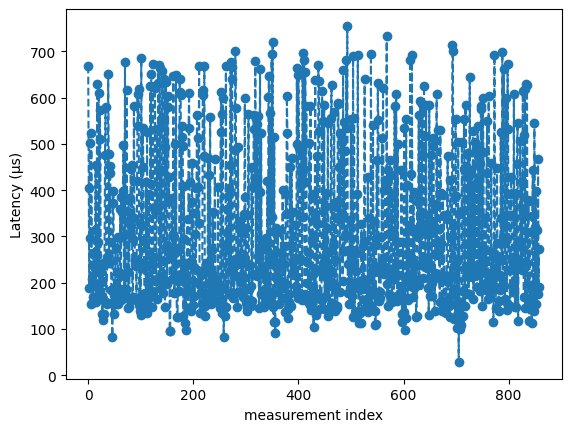
\includegraphics[width=1\linewidth]{img/Unbenannt.png}
    \caption{Latenz zwischen Erstellung des Eintrags und erstem Paket}
    \label{fig:placeholder}
\end{figure}
% Cite einfügen und begründen das größenordnung stimmt und angeben dass es eine BLueField 2 war.
Wie in der Abbildung 4.2 zu sehen ist, liegen die meisten Werte zwischen 150 und 250 $\mu s$. Der errechnete Median liegt bei \textbf{$249.8 \mu s$}. Die ausreißenden Minimalwerte sind wahrscheinlich dem Jitter der Hardware-Uhr auf Seiten der BlueField aufgrund der relativ kleinen Anzahl an Ausreißern zuzuordnen. Die hohen Maximalwerte können vernachlässigt werden, da sie durch den zufälligen Delay zustande kommen. Grundsätzlich wurde diesen gemessenen Werten innerhalb der Arbeitsgruppe glauben geschenkt, da sie sich mit der Veröffentlichung der Laconic-Gruppe deckten beziehungsweise in derselben Größenordnung lagen. Die Laconic-Arbeitsgruppe ermittelte einen Wert von $302 \mu s$ \cite{cui2024laconic}. Es sei allerdings erwähnt, dass sie einerseits auf der Bluefield-2 gemessen haben und andererseits bei dem Median aus diesem Projekt hier die Netzwerklatenz nicht abgezogen bzw. berücksichtigt wurde.
\section{Neuerungen in XenoFlow 1.0}
%\subsection{hash\_pipe}
% Siehe Doku einfügen
Die Einführung der Hash Pipe ist eine der größten Neuerungen und somit auch eines der Kernarbeitsziele dieses Projekts gewesen. Wie in Abschnitt 2.1.2 beschrieben, ermöglicht sie es, einen implizit ausgeführten Hashing Algorithmus auf die Netzwerkpakete anzuwenden. Implizit deshalb, da nicht explizit angegeben werden muss, wie der Hashing Algorithmus aufgebaut ist. Somit werden die Pakete gleichmäßig auf die entsprechenden Entries verteilt. 

Außerdem wurde in diesem Zug auch die Möglichkeit implementiert, dynamisch zur Laufzeit Backends hinzuzufügen und zu löschen. Dadurch ist eine genauere Anpassung des Loadbalancers in einer realen Einsatzsituation möglich, da bisher eine Änderung der Backends einen Neustart des Programms erfordern würde. Da dies mit entsprechendem Paketverlust einhergehen würde, war dieses Feature zu beginn des Praktikums im Fokus. Die Backends werden mittels einer REST-API auf dem Port 8080 hinzugefügt. Es kann mit jedem API-Call jeweils eine Anzahl von Backends hinzugefügt werden, sodass die neue Anzahl an Backends wieder einer Potenz von 2 entspricht. Im folgenden Code ist die entsprechende Funktion zum dynamischen hinzufügen eines Backends gegeben. Es sei dazu erwähnt, dass es sich um eine stark gekürzte Variante handelt. Die vollständige Version ist im Projekt Github-Repository einzusehen. Die entscheidenden aufgerufenen intrinsischen Funktionen sind hierbei:
\begin{itemize}
    \item \texttt{doca\_flow\_pipe\_hash\_add\_entry()} zum Erstellen des Entry, explizit in einer Hash-Pipe.
    \item \texttt{doca\_flow\_entries\_process()} ruft die Prozessierung in der Runtime auf (siehe 4.3).
\end{itemize}
\begin{minted}[linenos]{c}
doca_error_t xenoflow_add_backend(XenoFlow *xeno, char *name, char *mac) {
    int entry_index = xeno->config->numBackends;
    
    XenoFlowBackend *new_backend = createBackend(name, mac);
    doca_error_t result;
    
    SET_MAC_ADDR(actions.outer.eth.dst_mac,
        new_backend->mac_address[0], 
        new_backend->mac_address[1], 
        new_backend->mac_address[2],
        new_backend->mac_address[3], 
        new_backend->mac_address[4], 
        new_backend->mac_address[5]
    );
    
    fwd.type = DOCA_FLOW_FWD_PORT;
    fwd.port_id = 0;
    
    doca_flow_pipe_hash_add_entry(/* Entry Argumente */);
    doca_flow_entries_process(/* Entry Process Argumente */);
    
    configAddBackend(xeno->config, new_backend);
}
\end{minted}
Interessant ist hierbei die Zeile 19, da in dieser die intrinsische Funktion \texttt{doca\_flow\_pipe\_hash\_add\_entry()} verwendet wird. Es ist also nicht möglich, Entries mittels der vorherigen \texttt{doca\_flow\_pipe\_add\_entry()} in einer Hash-Pipe hinzuzufügen. Der Hintergrund ist vermutlich, dass beim Aufruf von \texttt{doca\_flow\_pipe\_hash\_add\_entry()} zusätzliche Funktionen aufgerufen werden müssen, um die entsprechenden Match-Masken neu aufzubauen. Diese Vermutung ist entstanden, da im Rahmen der Bachelorarbeit dieser Mechanismus selbst implementiert wurde und dadurch auffiel, dass bei einem Filtermechanismus, der als Eingabe \cite{heimbrodt2025bluefield} ein Bitfeld, also eine binäre Zahl, erhält, fast immer eine Anzahl von Filtern erstellt werden muss, die einer Potenz von 2 entspricht. Zuletzt wird in Zeile 22 der XenoFlow Konfiguration das neue Backend mittels \texttt{configAddBackend()} hinzugefügt. Dies geschieht, damit einerseits alle angelegten Backends in einer Datenstruktur gesammelt werden und somit beispielsweise auch Backends gelöscht werden können, aber auch, um eine Schnittstelle mit einem eventuellen Frontend/REST-API herstellen zu können.

Als HTTP-Server wurde im Projekt \textit{Micro HTTPD} verwendet. Diese Bibliothek ist extrem leichtgewichtig und ermöglicht es, schnell HTTP-Server aufzubauen, ohne große Teile des HTTP-Standards reimplementieren zu müssen.
\begin{minted}[linenos]{c}
int http_server_start(int port, XenoFlowConfig *config) {
    http_server_ctx = malloc(sizeof(struct http_server_ctx));    
    http_server_ctx->port = port;
    http_server_ctx->config = config;
    http_server_ctx->daemon = MHD_start_daemon(
        MHD_USE_SELECT_INTERNALLY,
        http_server_ctx->port,
        NULL, NULL,
        &http_request_handler, NULL,
        MHD_OPTION_END
    );
    // ... 
    DOCA_LOG_INFO("HTTP server started on port %d", http_server_ctx->port);
    return 0;
}
\end{minted}
In Zeile 5 wird der entsprechende Micro-HTTPD-Daemon gestartet und erhält als Callback-Funktion den entsprechenden Handler, in dem die eigentliche Verarbeitung stattfindet (Zeile 9). Die REST-API ermöglicht folgende Operationen:
\begin{itemize}
    \item GET gegen \texttt{/api-Pfad}: Gibt ein JSON zurück, das alle aktiven Backends enthält.
     \item POST gegen \texttt{/api}-Pfad: Erwartet eine Menge neuer Backends, die dem Loadbalancer hinzugefügt werden sollen.
\end{itemize}
Genauere Beispiele zum Format der JSON-Formatierung können im XenoFlow-Repository nachgelesen werden \cite{heimbrodt2025xenoflow}. Zum Parsen und Erstellen von JSON-Dateien wurde die Abhängigkeit \texttt{cJSON} dem Projekt hinzugefügt.

% weiter elaborieren was vollständig heißt
Die vorliegende Implementierung ermöglicht nun das Hinzufügen von Backends über die REST-API, ohne dass es zu Paketverlusten kommt. Das wird von Nvidia laut der eigenen Dokumentation garantiert. Damit rückt XenoFlow einem produktionsreifen System in signifikanter Weise näher. Die Funktionsweise des Hinzufügens von Backends wurde mittels einer eigenen Testumgebung überprüft. Das entsprechende Python Skript liegt ebenfalls im Projekt Repository vor.
\section{Sonstiges}
Zusätzlich zu den vorherigen Experimenten wurden weitere Features zum Loadbalancer und DOCA Flow allgemein hinzugefügt. Der Hintergrund war einerseits, Comfort-Features zu schaffen, die einer produktiven Nutzung helfen sollten, und andererseits, empfundene technische Lücken seitens Nvidia zu schließen.
\subsection{PyDFlow}
PyDFlow ist eine Python-Abstraktionsschicht, die es ermöglichen soll, Anwendungen für DOCA Flow und somit die BlueField in Python deutlich vereinfacht zu implementieren \cite{heimbrodt2025pydflow}. Ziel ist es, die Plattform auch für weniger komplexe Projekte sowie die Forschung attraktiver zu machen und technische Hürden zu verringern. Außerdem ist DOCA Flow aufgrund der Natur der C implementierung extrem verbose und neigt dazu, in sehr langem Programmcode für eigentlich simple Aufgaben zu münden. Daher soll PyDFlow die Möglichkeit bieten, schnelle Prototypen und forschungsorientierte Anwendungen für die BlueField-Flow-Plattform zu entwickeln. Das Projekt ist in C++ implementiert und verwendet das \textit{pybind11-Framework} \cite{jakob2015pybind11} zur Erstellung der Python bindings.
\begin{minted}[linenos]{python}
import pydflow

# Creating a DOCA Flow Pipe with the name test 
# and the PCIe addresses of Port 0 and Port 1 of the Bluefield
pyd = pydflow.PyDFlow("test", "03:00.0", "03:00.1")
pipe = pyd.create_pipe()
pipe.create_entry()

print(len(pipe.get_entries()))
print(pipe.get_entries())
\end{minted}
Zeile 1 zeigt, dass \texttt{pydflow} als ein C-Shared-Object gebaut wird und somit, dank der Fähigkeit von Python, C-Bibliotheken nahtlos einbinden zu können, als normale Python-Bibliothek importiert werden kann. In Zeile 5 wird die Umgebung von \texttt{PyDFlow} initialisiert und der Konstruktor erhält als Argumente einen Namen sowie die beiden PCIe-Adressen, auf denen die entsprechenden Pipes angelegt werden sollen.
In der nächsten Zeile und folgend (Zeilen 6-7) wird dann eine Pipe erstellt, der ein leeres Entry hinzugefügt wird.
Abschließend wird in den Zeilen 9 und 10 gezeigt, dass die erstellten Objekte vollständig in Python implementiert sind und spezifische Funktionen wie \texttt{len()} darauf ausgeführt werden können.
\subsection{Dashboard}
Da es nun üblich ist, alle webbezogenen Projekte auch mit einem Dashboard-Frontend auszustatten, wurde auch XenoFlow mit einem solchen Frontend ausgestattet. Dort können verschiedene Metrikwerte der entsprechenden Anwendung eingesehen werden.

Das Frontend wird als ein Python-Flask-Server gestartet, der in regelmäßigen Abständen mit dem Backend von XenoFlow kommuniziert, um den aktuellen Zustand auszulesen. Auf Abbildung 6.1 ist das Design des entsprechenden Frontends zu sehen. Dabei fragt %Python Json bla
% Zeitachse anfügen
\begin{figure}
    \centering
    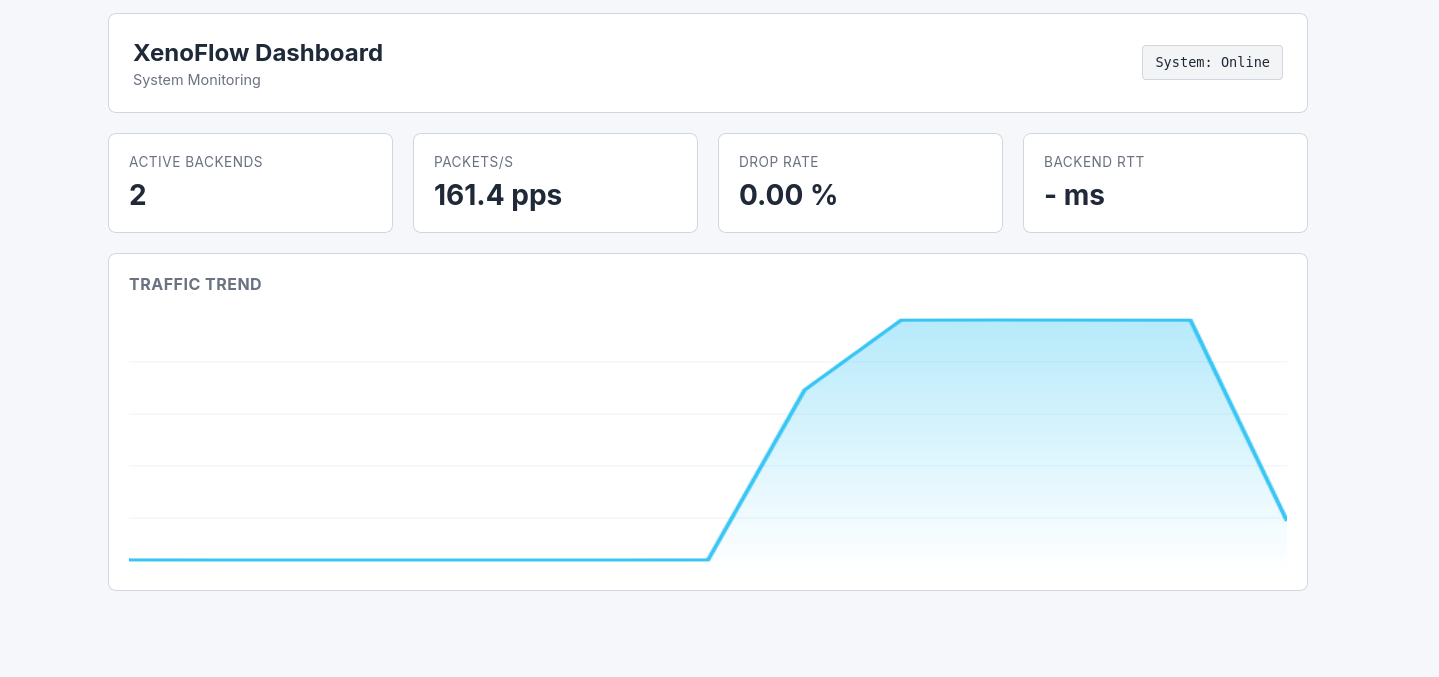
\includegraphics[width=1\linewidth]{img/dashboard.png}
    \caption{Dashboard des XenoFlow 1.0}
    \label{fig:placeholder}
\end{figure}
\section{Fazit}
% klareren Pfad zur 1.0 erläutern. Version 1.0 klar einführen (Einleitung)
Im Rahmen der Projektarbeit wurde XenoFlow vom ursprünglichen Zustand eines Prototypen ein gutes Stück weiter in die Richtung eines vollständigen Releases gebracht. Es konnten Erweiterungen für einen weiter ausgebauten, produktionsreifen Loadbalancer implementiert werden. So ist es nun in der Version 1.0 möglich, dynamisch zur Laufzeit neue Backends hinzuzufügen, die dann im Anschluss aktiv werden. Außerdem wurde der allgemeine Code wesentlich eingekürzt, da nun statt einer Filterfunktion und der entsprechenden Maskenberechnung einfach die DOCA Flow intrinsische Funktion aufgerufen wird. Dadurch ist keine Laufzeitsteigerung messbar, womit es sich um eine zero-cost-Erweiterung handelt. Damit ist nun das Projekt XenoFlow weitestgehend beendet. XenoFlow verbleibt als dynamisch konfigurierbarer L3 Loadbalancer. Es muss beim hinzufügen von Backends beachtet werden, dass stateful-TCP-Verbindungen korrekt wiederhergestellt werden müssen. Dies liegt dann allerdings nicht mehr in der obhut des Loadbalancers, sondern muss auf Applikationsebene gelöst werden. Abschließend lässt sich jedoch sagen, dass die technischen Gegebenheiten von ca. 4 Millionen Einträgen ($505 \text{ Pipes} \cdot 8192 \text{ Entries}$) und relativ geringen Entry-Einfüge-Latenzen von $249 \mu s$ eine gute Architektonische Grundlage für hardwarebeschleunigte Netzwerkpipelines bieten. \cite{heimbrodt2025bluefield}
\section{Ausblick}
\begin{figure}
    \centering
    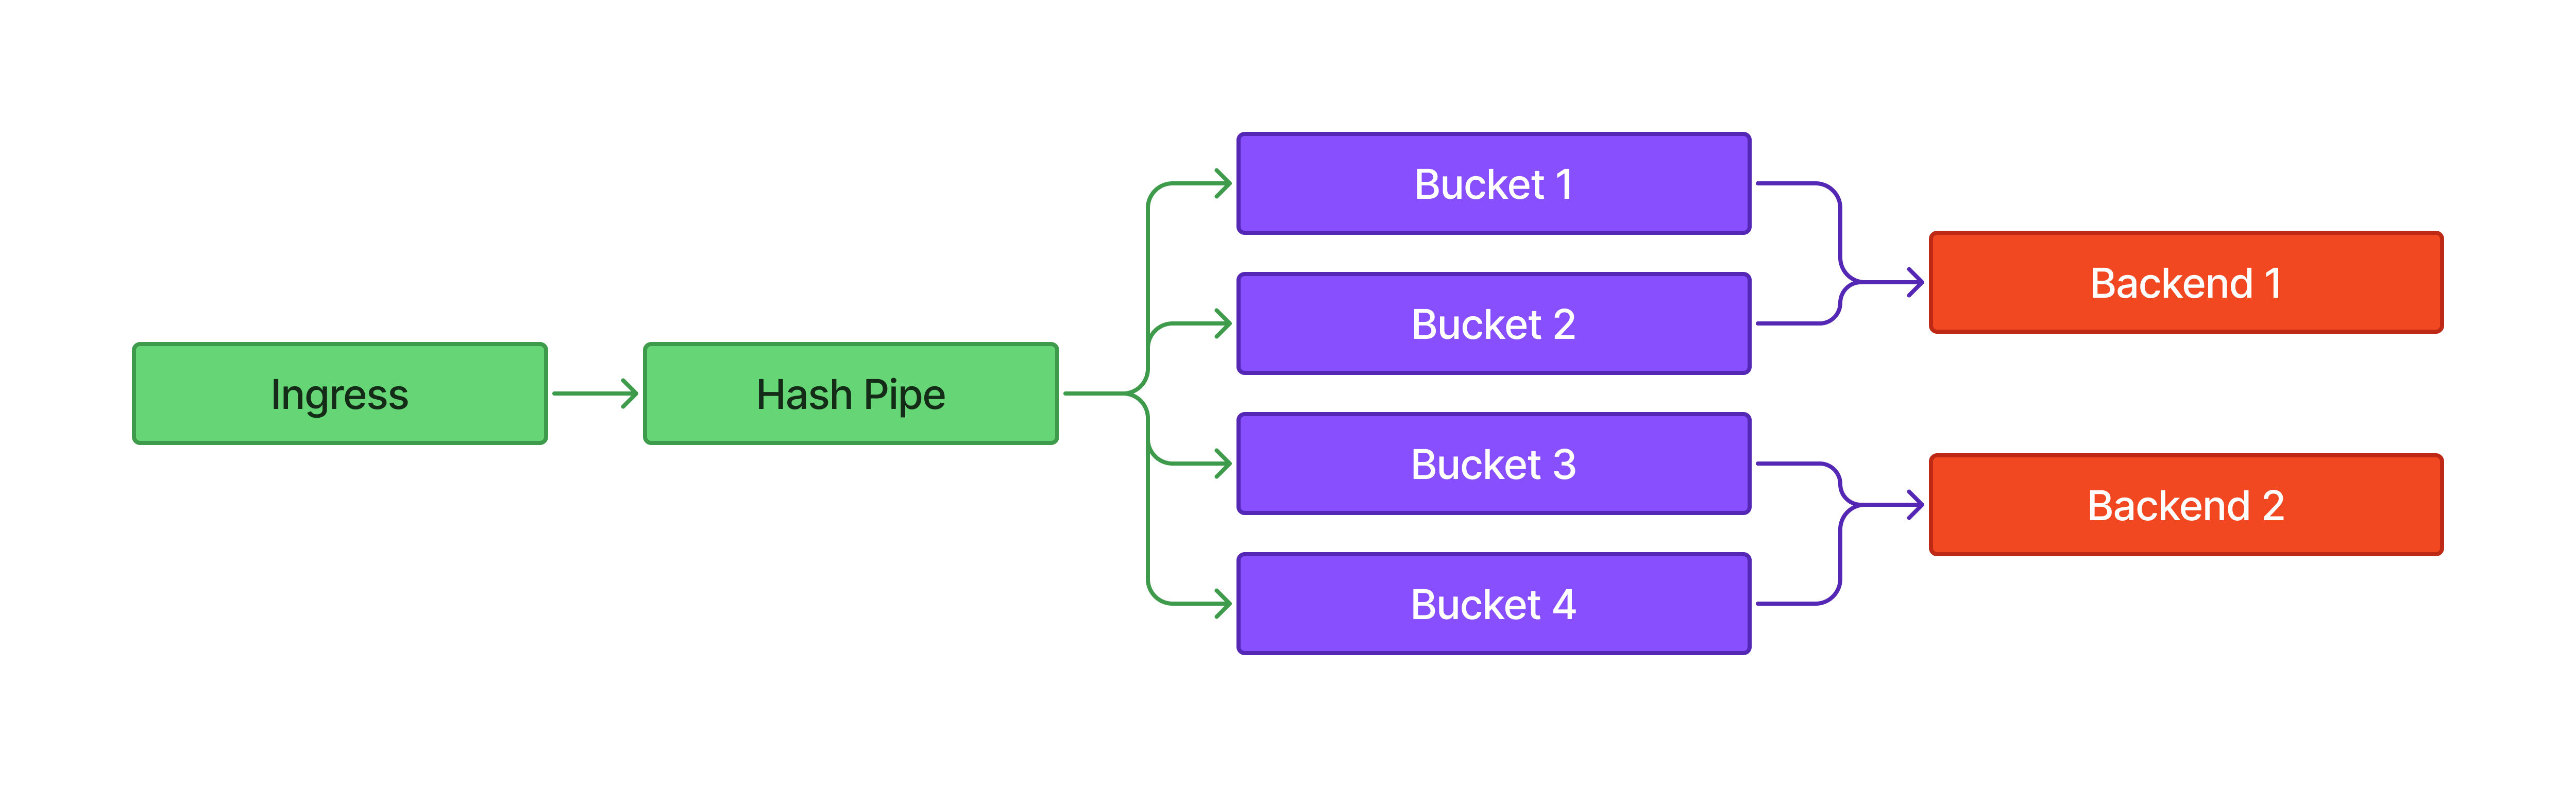
\includegraphics[width=1\linewidth]{img/Untitled.png}
    \caption{Bucket Semantik des Katran Loadbalancers \cite{shirokov2018katran}}
    \label{fig:placeholder}
\end{figure}
% Kein Konjunktiv 2
% Besser erklären wie Bucket und Backend Mappen vor allem im Bezug auf 7.1
% RSS Target einführen und Forwarding auf Flow beziehen
% Maglev einführen um auf Bucket hashing einzugehen
Das wohl größte fehlende Feature für XenoFlow wäre eine Per-Connection-Consistency. Dazu wäre es möglich, die Bucket Semantik von Katran nachzimplementieren. Die Idee ist es, zu ermöglichen, dass eine Anzahl von Backends, die nicht einer Zweierpotenz entspricht, abgebildet werden kann. Dabei wird, anstatt dass jedes Entry direkt auf ein Backend zeigt, eine feste Anzahl von Entries erstellt (Buckets). Die eigentliche Zuordnung, welches Bucket auf welches Backend zeigt, bleibt dann dem Programm überlassen. Dies ermöglicht es beispielsweise, einen 8 Bucket Zustand auch mit 3 Backends zu unterstützen (siehe Abbildung 7.1). Entscheidend sind jetzt hierbei die Backends, die noch eine laufende Stateful Verbindung mit einem Client geöffnet hatten. Dieser Traffic würde nach dem hinzufügen eines neuen Backends nicht mehr beim ursprünglichen Backend ankommen, da die entsprechenden Entries ja nun auf ein anderes Backend zeigen. Ein möglicher Weg, dies zu umgehen, wäre, den Traffic vorerst auf einen der ARM-Kerne mittels eines Forwarding an das RSS-Target zu schicken. Auf dem ARM Host werden dann entsprechend die laufenden Verbindungen explizit behandelt und mitgeschnitten. Nach einer gewissen Zeit wird ein Cut gemacht und die expliziten Verbindungen werden in einer Exception Pipe als expliziter Match hinzugefügt. Alle neuen Verbindungen werden von dieser Behandlung ausgenommen und werden direkt als klassische Verbindungen gehandhabt. Wichtig ist, dass der besagte Prozess abgeschlossen werden muss, bevor neue Backends hinzugefügt werden können. Einen ähnlichen Ansatz verfolgen wir im kommenden VeloxFlow \cite{schnoer2026veloxflow}. Dieser beschreibt einen Loadbalancer, der die QUIC Semantik unterstützt und zusätzlich die PCC für TCP implementieren soll.


\newpage
\printbibliography




























\end{document}